\documentclass[a4paper]{article} 
\addtolength{\hoffset}{-2.25cm}
\addtolength{\textwidth}{4.5cm}
\addtolength{\voffset}{-3.25cm}
\addtolength{\textheight}{5cm}
\setlength{\parskip}{0pt}
\setlength{\parindent}{0in}

\usepackage{natbib}
\usepackage{blindtext} % Package to generate dummy text
\usepackage{charter} % Use the Charter font
\usepackage[utf8]{inputenc} % Use UTF-8 encoding
\usepackage{microtype} % Slightly tweak font spacing for aesthetics
\usepackage{amsthm, amsmath, amssymb} % Mathematical typesetting
\usepackage{float} % Improved interface for floating objects
\usepackage{hyperref} % For hyperlinks in the PDF
\usepackage{graphicx, multicol} % Enhanced support for graphics
\usepackage{xcolor} % Driver-independent color extensions
\usepackage{pseudocode} % Environment for specifying algorithms in a natural way
\usepackage[ddmmyyyy]{datetime} % Uses YEAR-MONTH-DAY format for dates
%\usepackage{gensymb}
\usepackage{bibentry}

\usepackage{fancyhdr} % Headers and footers
\pagestyle{fancy} % All pages have headers and footers
\fancyhead{}\renewcommand{\headrulewidth}{0pt} % Blank out the default header
\fancyfoot[L]{} % Custom footer text
\fancyfoot[C]{} % Custom footer text
\fancyfoot[R]{\thepage} % Custom footer text
\newcommand{\note}[1]{\marginpar{\scriptsize \textcolor{red}{#1}}} % Enables comments in red on margin

%----------------------------------------------------------------------------------------

\usepackage{adjustbox}
\usepackage{float}
\usepackage{multicol}
\usepackage{pgfplots, pgfplotstable}
%-------------------------------
%	TITLE VARIABLES (identify your work!)
%-------------------------------

\newcommand{\yourname}{Jakob Kralj 4.A} % replace YOURNAME with your name
\newcommand{\papertitle}{Merjenje gostote kroglice} % replace X with paper title

\begin{document}

%-------------------------------
%	TITLE SECTION (do not modify unless you really need to)
%-------------------------------
\fancyhead[C]{}
\hrule \medskip
\begin{minipage}{0.295\textwidth} 
\raggedright
\footnotesize
\yourname \hfill\\ 
\end{minipage}
\begin{minipage}{0.69\textwidth} 
\centering 
\Large
\text{\papertitle}\\ 
\normalsize 
\end{minipage}
\medskip\hrule 
\bigskip


%-------------------------------
%	ASSIGNMENT CONTENT (add your responses)
%-------------------------------

\section*{Naloga:} % this is an example

Določi gostoto kroglic in jo zapiši z absolutno in relativno napako.

\section*{Potrebščine:}

Pet različno velikih kroglic iz istega materiala, kljunastno merilo, tehtnica

\section*{Skica:}
\begin{center}
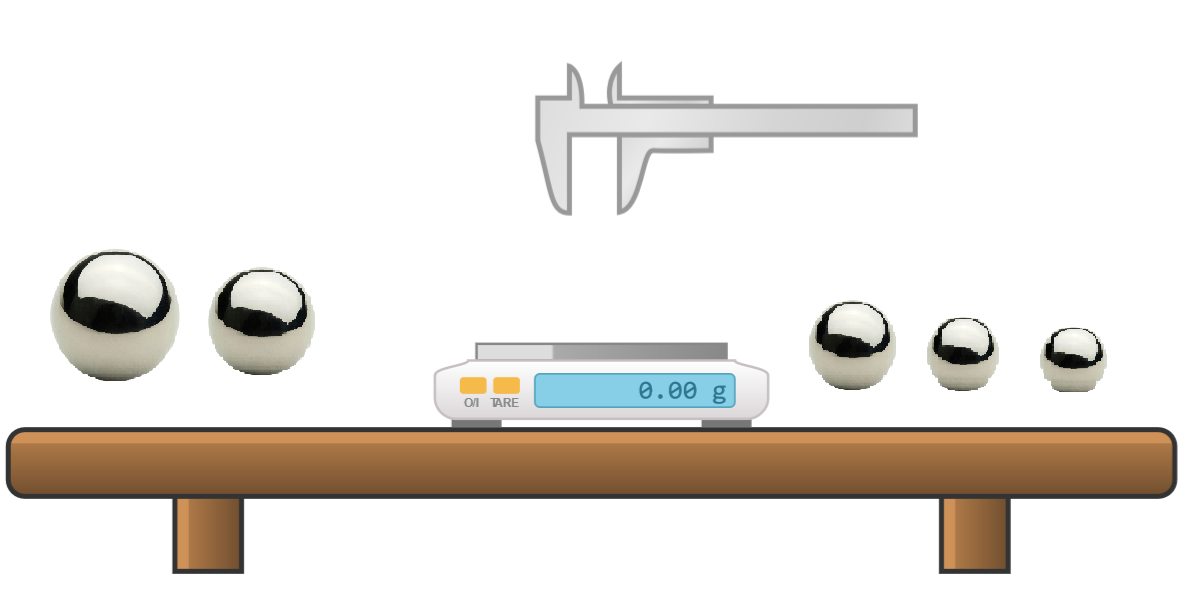
\includegraphics[scale=0.5]{skica.png}
\end{center}
\section*{Meritve:}

Stehtaj in izmeri premer vsake krogilice.

\begin{table}[H]
   \centering
\begin{tabular}{lll}
   & $d[mm]$ & $m[g]$ \\
   1 & 10     & 4,1  \\
   2 & 13     & 8,9  \\
   3 & 15     & 13,8 \\
   4 & 18     & 23,8 \\
   5 & 20     & 32,6
\end{tabular}
\end{table}



\section*{Rezultati in obdelava podatkov:}

\begin{multicols}{2}
$V$ lahko izračunamo s pomočjo formule:
\begin{equation}
   V = \frac{4\pi (\frac{d}{2})^3}{3}
\end{equation}

\columnbreak

$\rho$ lahko izračunamo s pomočjo formule:
\begin{equation}
   \rho = \frac{m}{V}
\end{equation}

\end{multicols}

Iz tega sledijo rezultati:
\begin{table}[H]
   \centering
\begin{tabular}{lllll}
   & $d[mm]$ & $m[g]$ & $V[mm^3]$ & $\rho[\frac{kg}{m^3}]$  \\
1 & 10     & 4,1  & 526         & 7795    \\
2 & 13     & 8,9  & 1150        & 7739    \\
3 & 15     & 13,8 & 1767        & 7810    \\
4 & 18     & 23,8 & 3054        & 7793    \\
5 & 20     & 32,6 & 4189        & 7782
\end{tabular}
\end{table}

Te rezultate lahko nanesemo tudi na graf $m(v)$:
\pgfplotstableread{
X Y
0.000000526 0.0041 
0.000001150 0.0089
0.000001767 0.0138
0.000003054 0.0238
0.000004189 0.0326
}\datatable

\begin{center}
\begin{tikzpicture}
\begin{axis}[
   legend pos= north west,
   title = {$m(V)$},
   xlabel={Prostornina $[m^3]$},
   ylabel={Masa $[kg]$}
   ]
\addplot [only marks, mark = *] table {\datatable};
\addplot [thick, red] table[
    y={create col/linear regression={y=Y}}
] % compute a linear regression from the input table
{\datatable};
\addlegendentry{$m(V)$}
\addlegendentry{%
$\pgfmathprintnumber{\pgfplotstableregressiona} \cdot x
\pgfmathprintnumber[print sign]{\pgfplotstableregressionb}$}
\end{axis}
\end{tikzpicture}
\end{center}

Strmina grafa je enaka gostoti, ki znaša $(7780 \pm 40) \frac{kg}{m^3}$ oz. $7780(1 \pm 0.005) \frac{kg}{m^3}$

Te rezultate lahko nanesemo tudi na graf $m(d)$:
\pgfplotstableread{
X Y
0.010 0.0041 
0.013 0.0089
0.015 0.0138
0.018 0.0238
0.020 0.0326
}\datatable

\begin{center}
\begin{tikzpicture}
\begin{axis}[
   legend pos= north west,
   title = {$m(d)$},
   xlabel={Premer $[m]$},
   ylabel={Masa $[kg]$},
   ]
\addplot [only marks, mark = *] table {\datatable};
\end{axis}
\end{tikzpicture}
\end{center}

Graf sledi obliki polinoma tretje stopnje. 

\section*{Dodatek}
Gostota kroglice ustreza večim kovinam, vendar pa bi glede na videz kroglic lahko sklepali da gre za jeklo. 
\section*{Interpretacija:}

Konstanti člen polinoma na grafu $m(V)$ je majhen (za okoli 9 redov velikost glede na prvi člen), kar pomeni da lahko sklepamo da gre premica skozi koordinatno izhodišče. To tudi nakazuje na relativno majhno relativno napako, kar pomeni da je bilo dela dokaj natančno.

\end{document}